%%%%%%%%%%%%%%%%%%%%%%%%%%%%%%%%%%%%%%%%%%%%%%%%%%%%%%%%%%%%%%%%%%%%%%%%
%                                                                      %
%     File: Simulation.tex		                                       %
%     Tex Master: Thesis.tex                                           %
%                                                                      %
%     Author: Israel Sother                                            %
%     Last modified: 27 May 2024                                       %
%                                                                      %
%%%%%%%%%%%%%%%%%%%%%%%%%%%%%%%%%%%%%%%%%%%%%%%%%%%%%%%%%%%%%%%%%%%%%%%%

\section{Simulation}
\label{section:simulation}%chktex 24
\vfill

To accelerate the development time, a model was developed in \textit{Simulink}, allowing for faster prototyping and direct comparison of the methods in a controlled environment. An adaptation of the \textit{Simscape Specialized Power Systems} block \textit{Permanent Magnet Synchronous Machine} was made to convert it to a delta-wound machine and to accept variable inductances as in \Cref{eq:motor_backward_euler_matrix}. 
This model was combined with six \glspl{mosfet} blocks in three legs to simulate the \gls{vsi}. To supply the \glspl{mosfet}, a model of the battery was made, where an ideal voltage source is connected through a series resistor to the DC link, where a capacitor stabilizes the voltage. In \Cref{fig:simulation_model} the resultant system is presented, where $S_1$, $S_2$, $S_3$, $S_4$, $S_5$, $S_6$, are the gate control signals that come from the control strategy.

\begin{figure}[!htb]
	\centering
	% \fbox{
		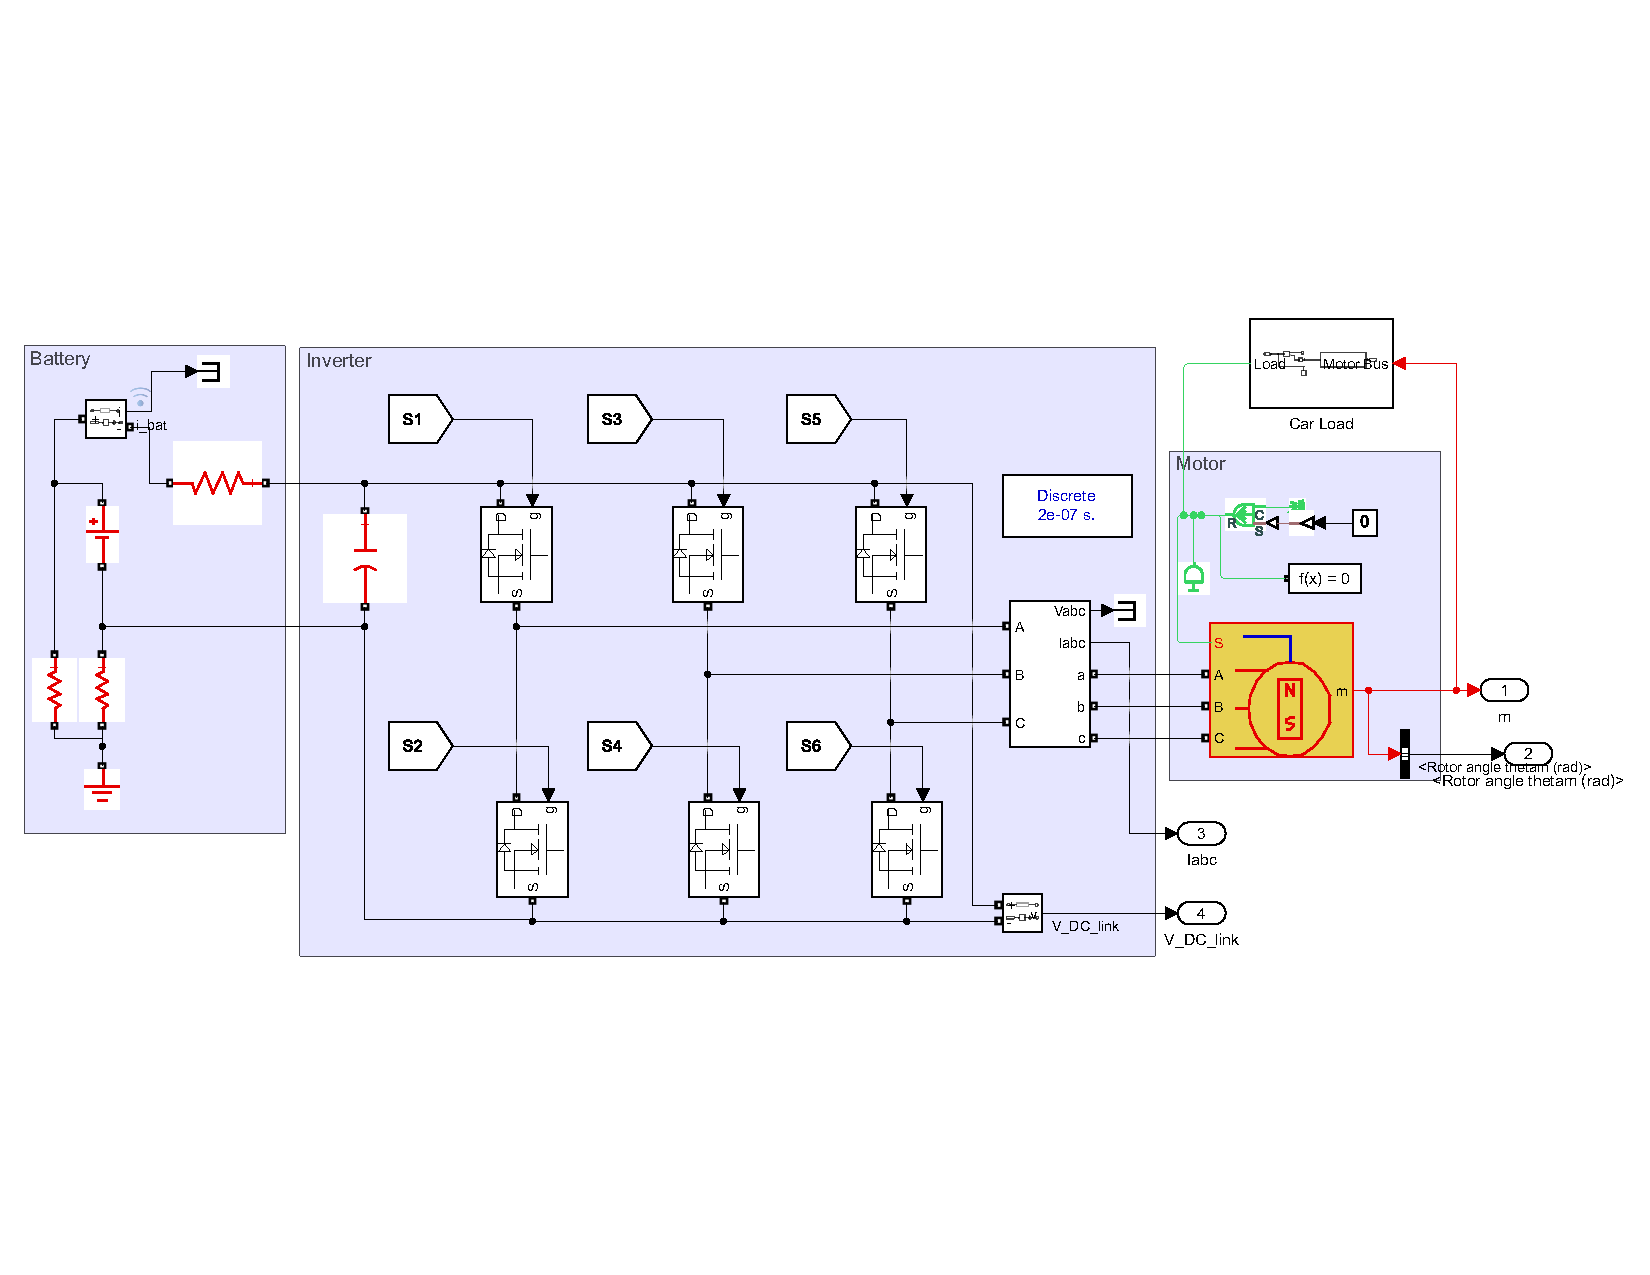
\includegraphics[clip, trim=0.3cm 5cm 0.5cm 5cm, width=1.00\textwidth]{Figures/motor_and_inverter_simulink1.pdf}
		% }
	\caption[Simulink Models, Motor and Inverter.]{Simulink Models, Motor and Inverter.}
	\label{fig:simulation_model} %chktex 24
\end{figure}

The parameterization of the \glspl{mosfet} used in the simulation is derived from the model used in~\cite{Costa:MSc}, the  Wolfspeed C2M0040120D. The motor model is the one derived on \Cref{section:PMSM model}, with the parameters from \Cref{section:motor_characterization}. The rotor position is based on Heidenhain ECI1118 properties as this is the encoder that the manufacturer uses. 
The DC link capacitor is set to $40\mu F$, while the battery series resistance is $0.03 \Omega$, both based on the existing hardware. The ground connections are $420k\Omega$ each, to simulate the isolation between high voltage and low voltage in the car, while the inertia and torque source blocks inside the motor area are to simulate the testbench environment, with the standard value of $0.0848 kg m^2$ to the inertia, and the torque source being controlled to maintain a constant speed. All those parameters are shown in \Cref{table:simulation_parameters} alongside the car parameters used in the load simulation on \Cref{section:acceleration}.

\begin{table}[h]
	\caption{Simulation Parameters}
	\label{table:simulation_parameters}%chktex 24
	\renewcommand{\arraystretch}{1.2} % more space between rows
	% \centering
	\begin{minipage}{0.49\textwidth}
		\centering
		\begin{tabular}{ll}
			\toprule
			\textbf{Simulation timestep} & $0.2\mu s$ \\\toprule
			\textbf{DC Link Capacitor} & $40\mu F$ \\\toprule
			\textbf{Battery Series Resistance} & $0.03 \Omega$ \\\toprule
			\textbf{Ground Connection} & $420k\Omega$ \\\toprule
			\textbf{Testbench Inertia} & $185 g cm^2$ \\\toprule
			\textbf{MOSFETs} & \begin{tabular}[c]{@{}l@{}}Wolfspeed \\ C2M0040120D\end{tabular} \\\toprule
			\textbf{Switching Frequency} & $50kHz$ \\\toprule
			\textbf{Encoder Resolution} & 18 bits \\\toprule
			\textbf{Encoder Frequency} & $12.5kHz$ \\\toprule
			\textbf{\begin{tabular}[c]{@{}l@{}}Current and Voltage \\ Sensor Resolution\end{tabular}} & 14 bits \\\toprule
			\textbf{\begin{tabular}[c]{@{}l@{}}Current and Voltage \\ Sensor Frequency\end{tabular}} & $50kHz$ \\\toprule
		\end{tabular}
	\end{minipage}
	% \hfill
	% \hspace{0.1cm}
	\begin{minipage}{0.49\textwidth}
		\centering
		\begin{tabular}{ll}
			\toprule
			\textbf{Car mass}                       & $230 kg$                      \\\toprule
			\textbf{Pilot mass}                     & $60 kg$                       \\\toprule
			\textbf{Tire radius}                    & $0.23 m$                      \\\toprule
			\textbf{\begin{tabular}[c]{@{}l@{}}Wheel assembly \\ moment of inertia\end{tabular}} & $0.2 kg m^2$ \\\toprule
			\textbf{Gear ratio}                     & $15.21$                       \\\toprule
			\textbf{Air density}                    & $1.2 kg/m^3$ \\\toprule
			\textbf{Reference car area}             & $1 m^2$      \\\toprule
			\textbf{Drag coefficient}               & $1.59$                        \\\toprule
			\textbf{Rolling resistance coefficient} & $0.09$                     \\\toprule
			\textbf{\begin{tabular}[c]{@{}l@{}}Speed Controller \\ proportional gain ($k_p$)\end{tabular}} & $0.035 Nm/rpm$ \\ \toprule
			\textbf{\begin{tabular}[c]{@{}l@{}}Speed Controller \\ integral gain ($k_i$)\end{tabular}}   & $10^{-9} Nm/rpm$ \\ \toprule
		\end{tabular}
	\end{minipage}
\end{table}

\subsection{Baseline Step}
With the model implemented on \textit{Simulink}, a baseline was made using the manufacturer control scheme, \gls{foc} with the standard $8kHz$ switching frequency, and compared with the proposed methods at $50kHz$. The difference in frequency is to account for the complete system, where the use of wide bandgap semiconductors allowed for a faster switching frequency. The baseline profile is a positive torque step with the machine fixed at the nominal speed of $12kRPM$. The rising time of each method is shown in \Cref{fig:rising_time_4_models}.
\begin{figure}[!htb]
	\centering
	\begin{subfigmatrix}{1}
		\subfigure[MPCs comparison. In orange the Finite set MPC, in yellow the finite set MPC with null vector, in green the continuous set implicit MPC, and in purple the proposed continuous set explicit MPC.]{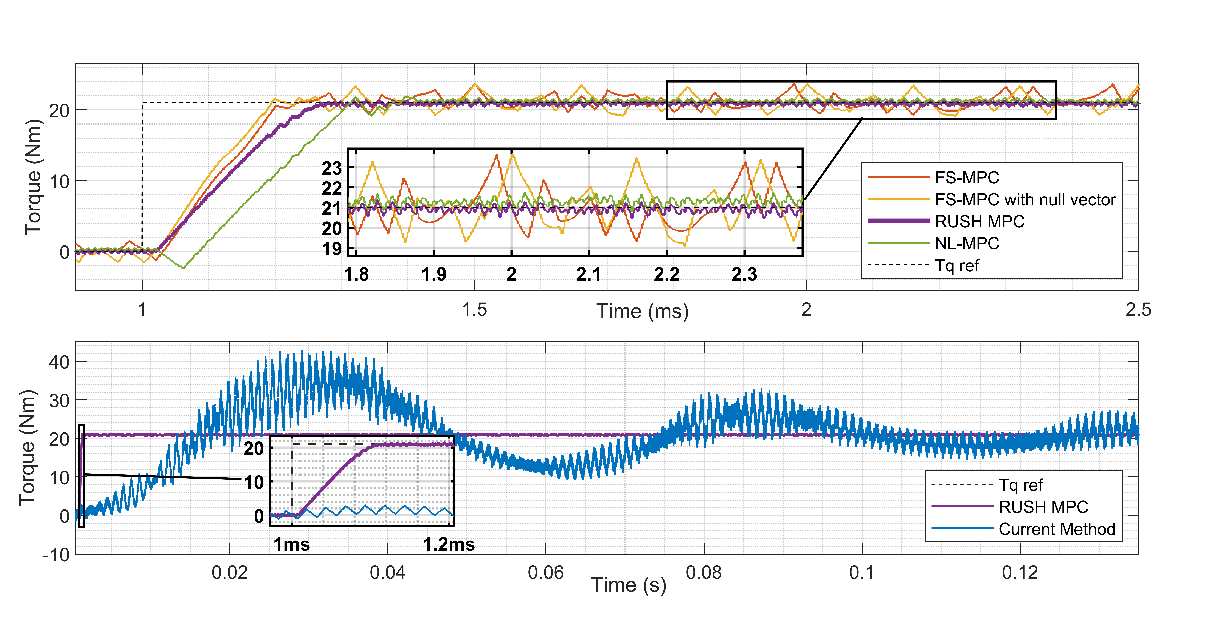
\includegraphics[clip, trim=0cm 4.8cm 0cm 0.75cm,width=1\textwidth]{Figures/Step_@12000RPM.eps}}
	\end{subfigmatrix}	
	\begin{subfigmatrix}{1}
		\subfigure[Proposed method (in purple) vs Currently used method (in blue).]{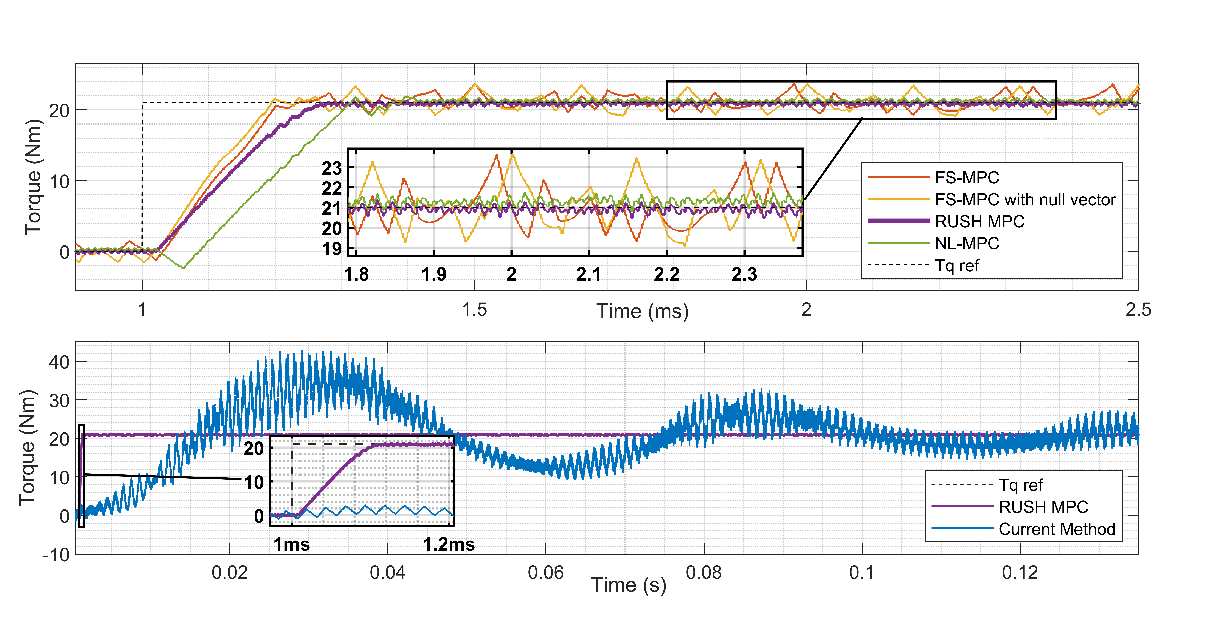
\includegraphics[clip, trim=0cm 0cm 0cm 5.5cm,width=1\textwidth]{Figures/Step_@12000RPM.eps}}
	\end{subfigmatrix}
	\caption[Control methods comparison in a torque step.]{Control methods comparison in a torque step.}
	\label{fig:rising_time_4_models} %chktex 24
\end{figure}

Note that the predictive controllers all perform similarly, having a good dynamic response, with an average rising time (0 to 100\%) of $200\mu s$, while the \gls{foc} method performed much slower, at approximately $180ms$. While the rising time in the \gls{foc} can be improved by better tuning the PID (these results are with the values recommended by the manufacturer), it would result in more pronounced overshoots and settling time, and would not reach the performance of a predictive controller, where the torque rising is only limited by the machine inductances, which shows the great dynamic performance of predictive controllers. It is important to also notice a small delay in the implicit \gls{nlmpc} response, this delay is due to the solver failing to converge. Although this may not always occur at each reference torque step, it was intentionally left on this graph to remind us of the possibility of this event. 

Divergence among the proposed methods becomes apparent during the analysis of steady-state conditions. The basic \gls{fsmpc} stands out with the highest torque and current ripple, significantly worse than the baseline, rendering it impractical. This ripple is due to the absence of a modulator, thus the chosen vector will stay applied for the full sampling time. Although an increase in switching frequency would improve the absolute performance of this method, in comparison it would never be as smooth as a modulated control, as it uses discrete vector options, while a simple \gls{svm} would switch multiple times in a single period. The increased switching reduces the ripple at the cost of lowered efficiency due to switching losses.

The addition of the null vector on the second method reduces the ripple at low angular speeds but still fails to do so when the machine accelerates, with curves very similar to the \gls{fsmpc}. The use of complete modulators can reduce this torque ripple problem, as the \gls{svm} allows for a third vector to be applied during the same time step, allowing the control to accurately point the voltage vector to the desired angle and amplitude, where the null vector only lets the controller change the amplitude of the existent active vectors.
\subsection{Current THD}

The distortion of currents was evaluated by setting the motor at a constant speed, waiting a few periods for it to reach a steady state and then calculating the average \gls{thd} of all line currents through 5 electrical periods. This was repeated in a grid pattern with some of the results shown in \Cref{table:thd_comparison}.

\begin{table}[h]
	\caption{Control Method Current THD comparison. THD is calculated until the Nyquist frequency, that is $250kHz$ and $40kHz$ for the controllers running at $50kHz$ and $8kHz$ respectively.}
	\label{table:thd_comparison}%chktex 24
	\renewcommand{\arraystretch}{1.2} % more space between rows
		\centering
		% \resizebox{1\textwidth}{!}{%
		\begin{tabular}{lrcccc}
			\textbf{} &
			  \multicolumn{1}{l}{\textbf{}} &
			  \textbf{1000 RPM} &
			  \textbf{7333 RPM} &
			  \textbf{13666 RPM} &
			  \textbf{20000 RPM} \\ \toprule
			 &
			  \textbf{1Nm} &
			  57.62\% &
			  43.44\% &
			  207.54\% &
			  29.62\% \\
			 &
			  \textbf{11Nm} &
			  3.22\% &
			  10.62\% &
			  12.14\% &
			  58.53\% \\
			\multirow{-3}{*}{\textbf{\begin{tabular}[c]{@{}l@{}}FOC \\ @8kHz\end{tabular}}} &
			  \textbf{20Nm} &
			  5.15\% &
			  6.50\% &
			  10.18\% &
			  37.08\% \\ \toprule
			 &
			  \textbf{1Nm} &
			  56.95\% &
			  11.08\% &
			  14.12\% &
			  4.71\% \\
			 &
			  \textbf{11Nm} &
			  2.18\% &
			  2.19\% &
			  1.93\% &
			  4.85\% \\
			\multirow{-3}{*}{\textbf{\begin{tabular}[c]{@{}l@{}}FOC \\ @50kHz\end{tabular}}} &
			  \textbf{20Nm} &
			  1.41\% &
			  1.41\% &
			  2.28\% &
			  3.86\% \\ \toprule
			 &
			  \textbf{1Nm} &
			  696.41\% &
			  566.94\% &
			  247.13\% &
			  72.31\% \\
			 &
			  \textbf{11Nm} &
			  39.42\% &
			  30.17\% &
			  28.04\% &
			  11.82\% \\
			\multirow{-3}{*}{\textbf{\begin{tabular}[c]{@{}l@{}}FS-MPC \\ @50kHz\end{tabular}}} &
			  \textbf{20Nm} &
			  22.10\% &
			  16.88\% &
			  8.52\% &
			  11.82\% \\ \toprule
			 &
			  \textbf{1Nm} &
			  30.67\% &
			  120.31\% &
			  159.20\% &
			  221.12\% \\
			 &
			  \textbf{11Nm} &
			  1.59\% &
			  10.65\% &
			  12.40\% &
			  11.51\% \\
			\multirow{-3}{*}{\textbf{\begin{tabular}[c]{@{}l@{}}FS-MPC \\ Null Vector \\ @50kHz\end{tabular}}} &
			  \textbf{20Nm} &
			  1.76\% &
			  6.43\% &
			  7.10\% &
			  8.54\% \\ \toprule
			 &
			  \textbf{1Nm} &
			  6.59\% &
			  9.98\% &
			  12.60\% &
			  14.50\% \\
			 &
			  \textbf{11Nm} &
			  0.81\% &
			  1.48\% &
			  1.89\% &
			  2.17\% \\
			\multirow{-3}{*}{\textbf{\begin{tabular}[c]{@{}l@{}}NL-MPC \\ @50kHz\end{tabular}}} &
			  \textbf{20Nm} &
			  0.81\% &
			  0.96\% &
			  1.18\% &
			  1.12\% \\ \bottomrule
			 &
			  \textbf{1Nm} &
			  7.20\% &
			  11.91\% &
			  16.82\% &
			  21.95\% \\
			 &
			  \textbf{11Nm} &
			  0.76\% &
			  1.47\% &
			  1.92\% &
			  2.16\% \\
			\multirow{-3}{*}{\textbf{\begin{tabular}[c]{@{}l@{}}RUSH MPC \\ @50kHz\end{tabular}}} &
			  \textbf{20Nm} &
			  0.81\% &
			  0.98\% &
			  1.19\% &
			  1.12\% \\ \toprule
			\end{tabular}
		% }
\end{table}

Table \ref{table:thd_comparison} exposes the advantage of continuous \gls{mpc} over the other alternatives, with distortions expressively smaller than the baseline and the finite set \glspl{mpc}, backing up the ripple analysis previously made. As expected the addition of a null vector reduced expressively the \gls{thd} in operation points of low modulation index, but made no difference when the modulation index increased. When comparing the methods that use \gls{svm}, the distortion is very similar when operated at the same frequency, meaning that the main factor is the modulation frequency, not the control algorithm.

Another advantage of the proposed methods is they actively use the direct axis current to generate torque throughout the full operation map of the motor,  not only in field weakening as the method currently implemented on the car. This is a result of the use of \gls{mtpa} references which improves efficiency, as it produces a reduction in the current vector modulus necessary to generate the same torque.
\subsection{Robustness}

To test the controller's robustness, a Monte Carlo analysis is proposed. A normal distribution is assigned to the motor parameters with a mean equal to the characterized value, and a standard deviation equal to 5\% of the mean. The step of \Cref{fig:rising_time_4_models} was simulated for 1000 samples with the modified parameters applied to the motor without updating the controller (\Cref{fig:montecarlo}).

\begin{figure}[!htb]
	\centering
	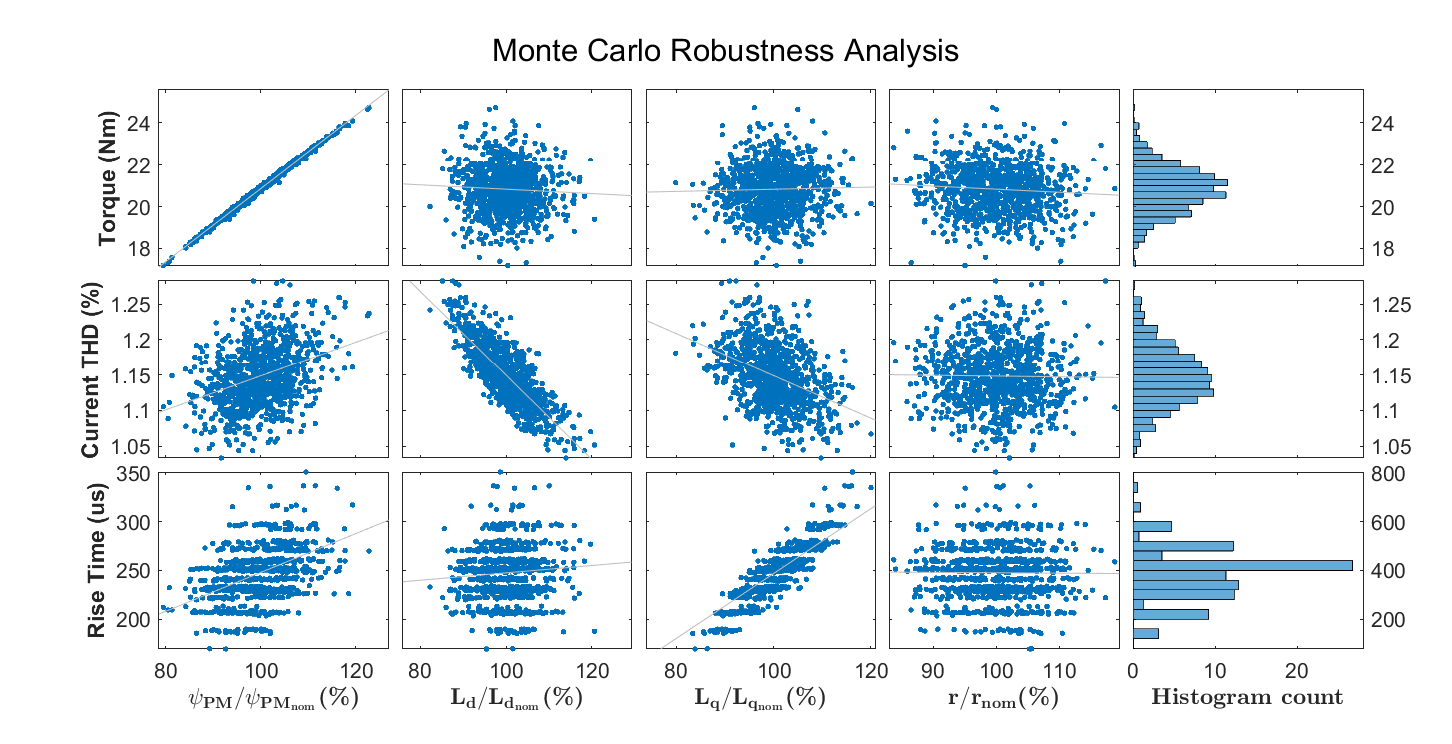
\includegraphics[width=1\textwidth]{Figures/MonteCarlo.eps}
	\caption[Monte Carlo Robustness Analysis.]{Monte Carlo Robustness Analysis. The motor parameters are shown in percentual change from the controller's expected value.}
	\label{fig:montecarlo} %chktex 24
\end{figure}

To evaluate the performance with degraded parameters three metrics were used, the steady-state mean torque, the steady-state current \gls{thd}, and the torque rising time. Based on these metrics the most influential parameter is the flux linkage, with a correlation of almost 100\% with the steady-state torque as shown in \Cref{fig:corr_plot}. This is explained by the type of motor used, where the inductances between the direct and quadrature axes are very similar, resulting in most of the torque derived from the permanent magnet's flux linkage. Note that this dependency is also present in the method currently used by the team, where the quadrature current reference is based on the machine torque constant ($k_t$). 
While relatively easy to characterize, the flux linkage is also the parameter most prone to change with the life of the motors, where the magnets can overheat or be demagnetized by a high direct axis current, thus a good approach is to develop a characterization routine that can be automatically executed whenever the user deems necessary.

\begin{figure}[!htb]
	\begin{subfigmatrix}{2}
		\subfigure[Steady State Torque]{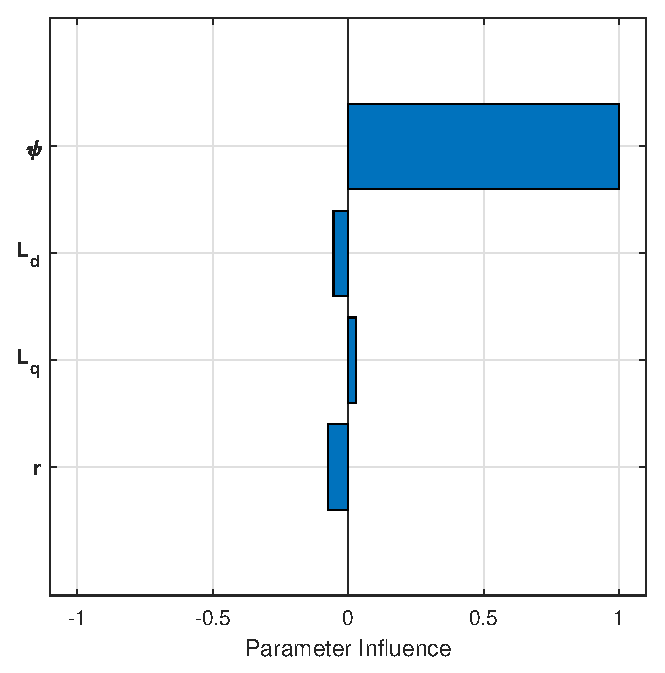
\includegraphics[width=0.4\linewidth]{Figures/corr_tq.eps}\label{fig:corr_tq}}
		\subfigure[Current THD]{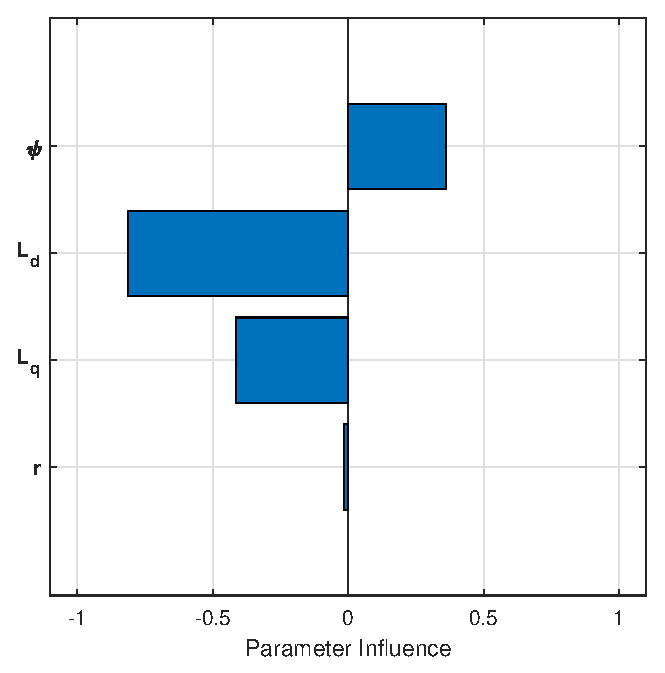
\includegraphics[width=0.4\linewidth]{Figures/corr_thd.eps}\label{fig:corr_thd}}
	\end{subfigmatrix}
	\begin{subfigmatrix}{1}
		\subfigure[Torque Rise Time]{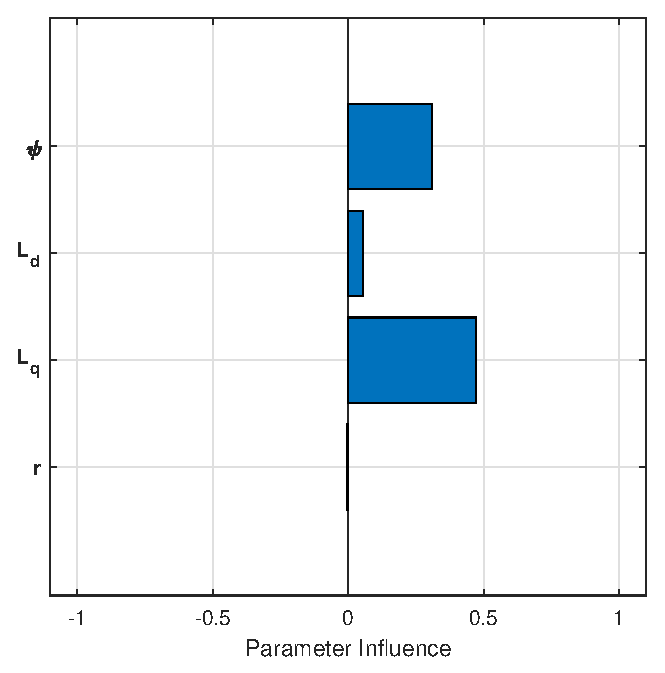
\includegraphics[width=0.4\linewidth]{Figures/corr_risetime.eps}\label{fig:corr_risetime}}
	\end{subfigmatrix}
	\caption{Parameter correlation coefficient with performance metrics.}
	\label{fig:corr_plot}%chktex 24
\end{figure}

The quadrature inductance has a higher correlation with the torque rise time, as expected. Since almost all of the torque is derived from the permanent magnet's flux linkage the torque will rise as fast as the controller manages to create quadrature currents. While this correlation is not definitive proof, it reinforces the statement that the proposed controller dynamic response is limited by the machine inductances. The high flux linkage correlation with the rise time is due to the increase in steady-state torque since with higher flux the steady-state torque is higher and the rise is approximately linear, with an increase in steady-state torque the rise time also increases.

Regarding the current \gls{thd}, the parameter influences are well balanced, with the direct axis inductance being a little more correlated. When combining this with the small absolute variance of the \gls{thd}, it is clear that the control strategy is very robust against model mismatches, maintaining a low distortion even with the wrong parameters.

\subsection{Acceleration Event}
\label{section:acceleration}%chktex 24

The load profile defined in \Cref{section:03load_profile} was used to simulate a typical acceleration event. The car load parameters are as shown in \Cref{table:simulation_parameters}, and the torque reference was set to reach $21.3kW$ of delivered power (after inverter and motor efficiency losses). The power value was chosen assuming an $80\%$ powertrain efficiency and the previous approximation of one-third of the car load on the rear motors. As shown in \Cref{fig:acceleration_comparison}, the \gls{rush} improved the time from $3.943s$ to $3.883s$ ($1.6\%$), reaching also a higher top speed than the currently implemented control method and presenting a lower torque ripple. While the $0.06s$ seems like a small gain, comparing with the results from \gls{fsg} 2023 it would put \gls{fst} three positions higher in the event ranking. If the proposed control method is combined with the efficiency improvement from the use of new inverter hardware, the time is further reduced, to $3.759s$ ($4.7\%$), translating to a 6 position gain in the event ranking.

\begin{figure}[!htb]
	\centering
	\begin{subfigmatrix}{2}
		\subfigure[Torque profile in the acceleration event using the currently implemented FOC.]{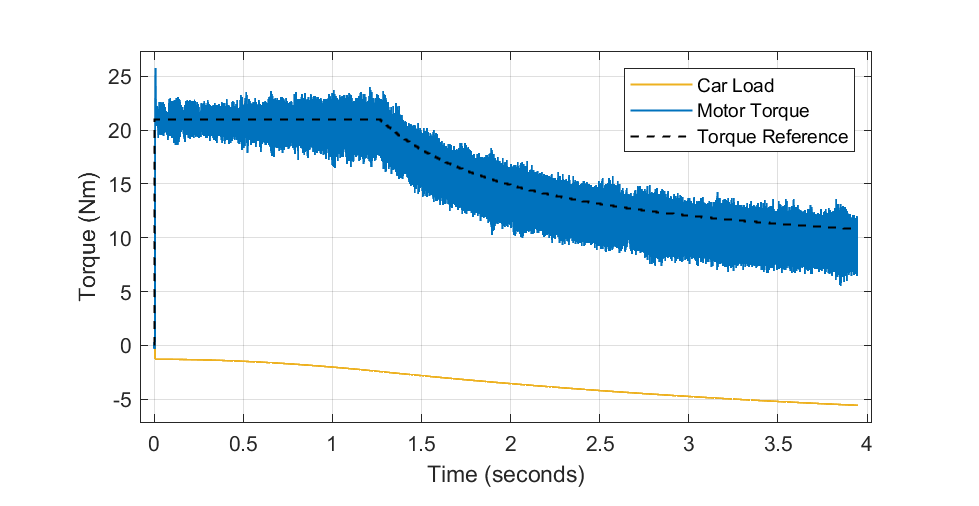
\includegraphics[clip,trim = 1cm 0 1.55cm 0,width=0.49\linewidth]{Figures/acc_empc.eps}\label{fig:acc_foc}}
		\subfigure[Torque profile in the acceleration event using the proposed EMPC]{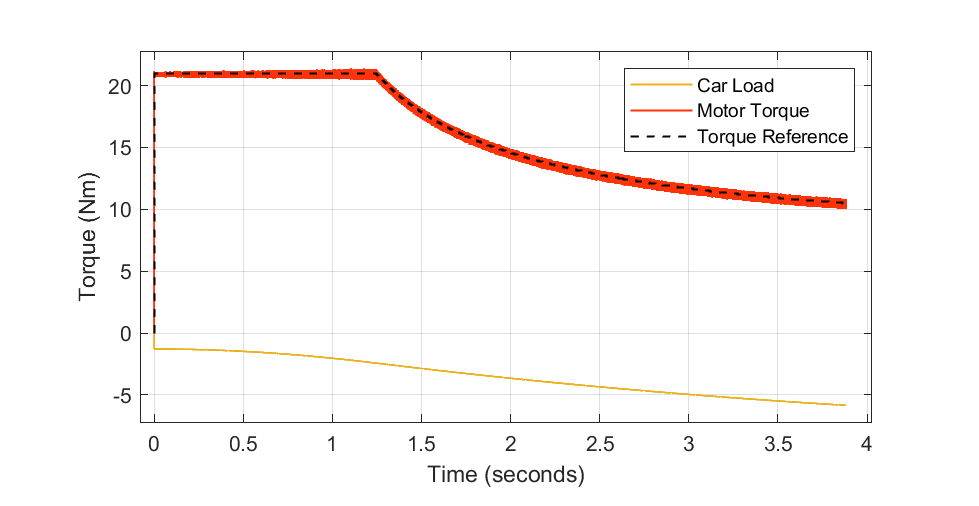
\includegraphics[clip,trim = 1cm 0 1.55cm 0,width=0.49\linewidth]{Figures/acc_foc.eps}\label{fig:acc_empc}}
	\end{subfigmatrix}
	\begin{subfigmatrix}{2}
		\subfigure[Motor speed profile in the acceleration event. The blue line is the currently implemented FOC while the orange line is the proposed EMPC.]{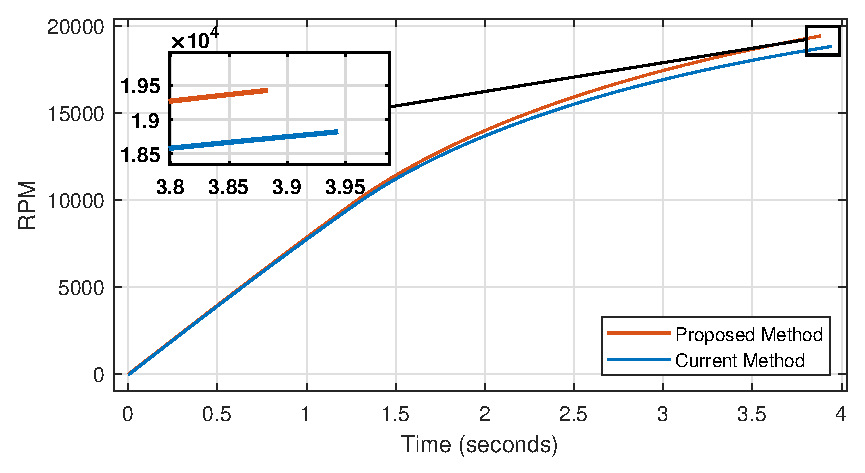
\includegraphics[width=0.49\linewidth]{Figures/acc_rpm.eps}\label{fig:acc_rpm}}
		\subfigure[Distance traveled in the acceleration event. The blue line is the currently implemented FOC while the orange line is the proposed EMPC.]{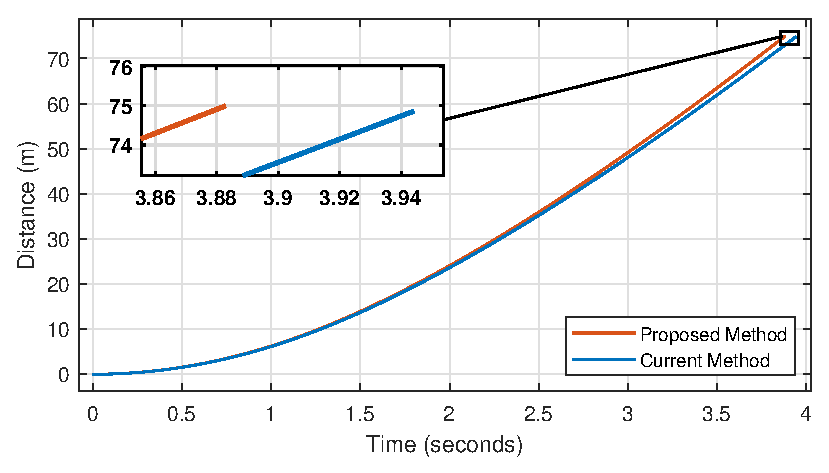
\includegraphics[width=0.475\linewidth]{Figures/acc_dist.eps}\label{fig:acc_dist}}
	\end{subfigmatrix}
	\caption[Control methods comparison on an Acceleration event.]{Control methods comparison on an Acceleration event.}
	\label{fig:acceleration_comparison} %chktex 24
\end{figure}